
    %%%%% %%%%% %%%%%
    %               %
    % New row       %
    %               %
    %%%%% %%%%% %%%%%
\begin{columns}[t]
  \begin{column}{0.71\textwidth}
    \begin{block}{\large A model for emergence}
      \begin{columns}
        \begin{column}{0.55\textwidth}
%\small
\footnotesize
%\tiny
Most emergences of \textit{P. infestans} may be ephemeral.
Occasional emergence of high fitness lineages displace preceding lineages.
Our work shows that these high fitness clones are also associated with high CNV.
This research also indicates a link between a copy number of two and a sexual mode of reproduction.
It is currently unknown whether a copy number of three drives fitness or it accumulates after highly fit lineages emerge.
It is also unknown if lineages of high copy number can revert back to a copy number of two.
        \end{column}
        \begin{column}{0.44\textwidth}
          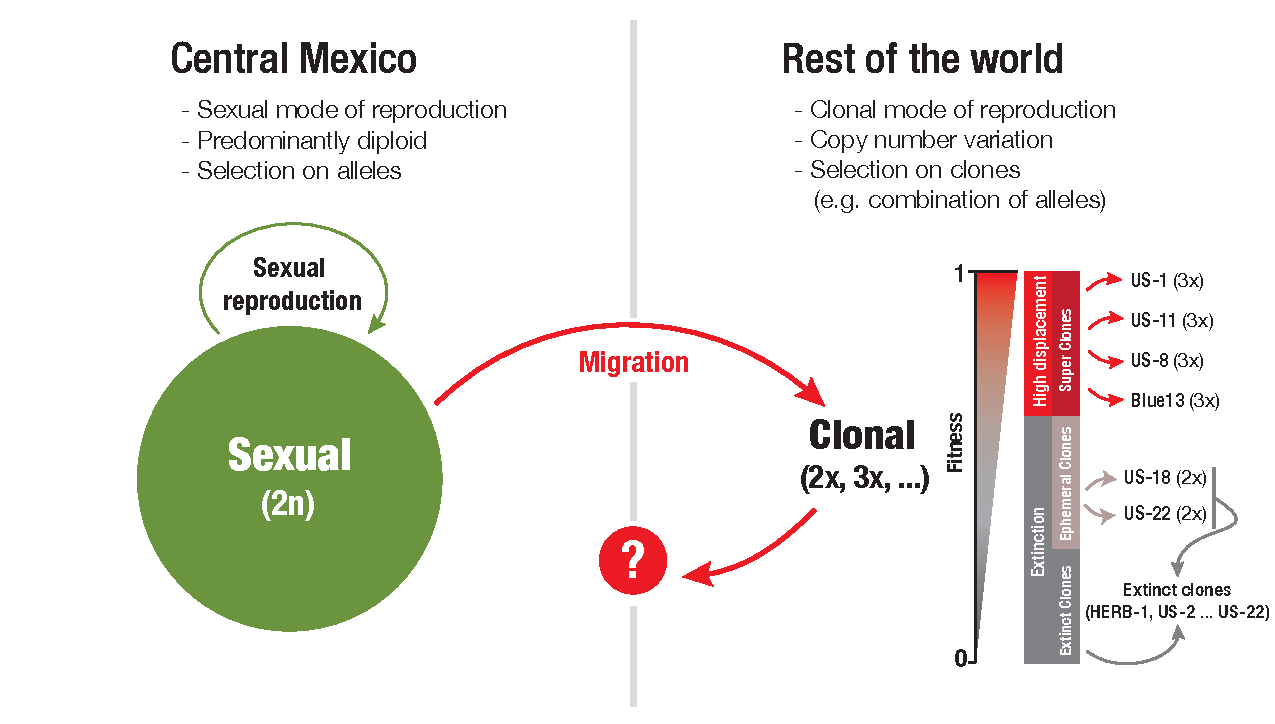
\includegraphics[height=20cm]{./figures/Fig8_Model.pdf}
        \end{column}
      \end{columns}

    \end{block}
  \end{column}

  \begin{column}{0.22\textwidth}
    \begin{block}{\large Acknowledgments}
\tiny
\vspace{10mm}

This research is supported in part by USDA National Institue of Food and Agriculture Grant 2011-68004-30154.
\newline
\vspace{5mm}

\textbf{References}\\
Knaus, B. J., \& Gr\"unwald, N. J. (2018). Inferring variation in copy number using high throughput sequencing data in R. Frontiers in Genetics, 9.
\newline
\vspace{1cm}

vcfR can be found at:
https://CRAN.R-project.org/package=vcfR
\vspace{1cm}

    \end{block}
  \end{column}
\end{columns}


